\newcommand{\spywareTagResultsAucTable}{
    \begin{table}[H]
        \centering
        \begin{tabular}{|p{2,8cm}||p{2,8cm} p{2,8cm} p{2,8cm}|}
            \hline
            Spyware Tag & ALOHA & Joint Embedding & Proposed Model \\
            \hline
            AUC-ROC & 0.604$\pm$0.159 & \textBF{0.662$\pm$0.014} & 0.584$\pm$0.076 \\
            \hline
        \end{tabular}
        \caption{AUC-ROC (Area Under Curve) of the different models for the \textbf{Spyware Tag} prediction task. Results were aggregated over \textBF{3} training runs with different weight initializations and minibatch orderings. Best results are shown in \textbf{bold}.} \label{tab:spywareTag_auc}
    \end{table}
}

\newcommand{\spywareTagResultsAtFprTable}{
    \begin{center}
        \begin{longtable}[c]{|p{3,2cm}||p{1,8cm} p{1,8cm} p{1,8cm} p{1,8cm} p{1,8cm}|}
            \hline
            Spyware Tag & \multicolumn{5}{c|}{{FPR}} \\
            & $10^{-5}$ & $10^{-4}$ & $10^{-3}$ & $10^{-2}$ & $10^{-1}$ \\
            \hline
            \endfirsthead

            \caption*{\raggedright ...continued from previous page} \\
            \hline
            Spyware Tag & \multicolumn{5}{c|}{\textbf{FPR}} \\
            & $10^{-5}$ & $10^{-4}$ & $10^{-3}$ & $10^{-2}$ & $10^{-1}$ \\
            \hline
            \endhead

            \caption*{\raggedleft ...continued on next page} \\
            \endfoot

            \caption{Mean and standard deviation results (TPR, Accuracy, Recall, Precision and F1-Score) of the different models for the \textbf{Spyware Tag} prediction task at different \textbf{FPR}s (\textit{False Positive Rates}). Results were aggregated over \textBF{3} training runs with different weight initializations and minibatch orderings. Best results are shown in \textbf{bold}. Under \textbf{TPR} results are also presented the percentage reduction in mean detection error and in ROC curve standard deviation introduced by the \textit{Proposed Model} with respect to both \textit{ALOHA} model and \textit{Joint Embedding}.} \label{tab:spywareTag_results_at_fpr} \\
            \endlastfoot

            \multicolumn{6}{|c|}{\textbf{TPR}} \\
            \hline
            ALOHA & 0.007$\pm$0.010 & 0.007$\pm$0.010 & 0.016$\pm$0.013 & 0.057$\pm$0.017 & 0.256$\pm$0.115 \\
            Joint Embedding & 0.033$\pm$0.003 & 0.034$\pm$0.003 & 0.053$\pm$0.000 & 0.103$\pm$0.062 & 0.256$\pm$0.060 \\
            Proposed Model & \textBF{0.039$\pm$0.014} & \textBF{0.039$\pm$0.014} & \textBF{0.079$\pm$0.039} & \textBF{0.136$\pm$0.060} & \textBF{0.275$\pm$0.048} \\
            \hline
            Error Reduction wrt \newline ALOHA & 3.2\% & 3.2\% & 6.4\% & 8.4\% & 2.6\% \\
            Error Reduction wrt \newline Joint Embedding & 0.6\% & 0.5\% & 2.7\% & 3.7\% & 2.6\% \\
            \hline
            Std Reduction wrt \newline ALOHA & -40.0\% & -40.0\% & -200.0\% & -252.9\% & 58.3\% \\
            Std Reduction wrt \newline Joint Embedding & -366.7\% & -366.7\% & 0.0\% & 3.2\% & 20.0\% \\
            \hline
            \multicolumn{6}{|c|}{\textbf{Accuracy}} \\
            \hline
            ALOHA & 0.871$\pm$0.001 & 0.871$\pm$0.001 & 0.871$\pm$0.002 & 0.869$\pm$0.002 & 0.816$\pm$0.015 \\
            Joint Embedding & 0.874$\pm$0.000 & 0.874$\pm$0.000 & 0.876$\pm$0.000 & 0.876$\pm$0.007 & 0.815$\pm$0.010 \\
            Proposed Model & \textBF{0.875$\pm$0.002} & \textBF{0.875$\pm$0.002} & \textBF{0.879$\pm$0.005} & \textBF{0.878$\pm$0.009} & \textBF{0.819$\pm$0.006} \\
            \hline
            \multicolumn{6}{|c|}{\textbf{Recall}} \\
            \hline
            ALOHA & 0.007$\pm$0.010 & 0.007$\pm$0.010 & 0.016$\pm$0.013 & 0.057$\pm$0.017 & 0.256$\pm$0.115 \\
            Joint Embedding & 0.033$\pm$0.003 & 0.033$\pm$0.003 & 0.053$\pm$0.000 & 0.103$\pm$0.062 & 0.256$\pm$0.060 \\
            Proposed Model & \textBF{0.039$\pm$0.014} & \textBF{0.039$\pm$0.014} & \textBF{0.079$\pm$0.039} & \textBF{0.136$\pm$0.060} & \textBF{0.275$\pm$0.048} \\
            \hline
            \multicolumn{6}{|c|}{\textbf{Precision}} \\
            \hline
            ALOHA & \textBF{1.000$\pm$0.000} & \textBF{1.000$\pm$0.000} & 0.556$\pm$0.393 & 0.469$\pm$0.057 & 0.265$\pm$0.101 \\
            Joint Embedding & \textBF{1.000$\pm$0.000} & \textBF{1.000$\pm$0.000} & 0.895$\pm$0.000 & \textBF{0.620$\pm$0.104} & 0.272$\pm$0.052 \\
            Proposed Model & \textBF{1.000$\pm$0.000} & \textBF{1.000$\pm$0.000} & \textBF{0.913$\pm$0.030} & 0.620$\pm$0.156 & \textBF{0.291$\pm$0.033} \\
            \hline
            \multicolumn{6}{|c|}{\textbf{F1 Score}} \\
            \hline
            ALOHA & 0.014$\pm$0.020 & 0.014$\pm$0.020 & 0.030$\pm$0.025 & 0.102$\pm$0.029 & 0.260$\pm$0.109 \\
            Joint Embedding & 0.065$\pm$0.006 & 0.065$\pm$0.006 & 0.101$\pm$0.000 & 0.173$\pm$0.094 & 0.264$\pm$0.056 \\
            Proposed Model & \textBF{0.074$\pm$0.026} & \textBF{0.074$\pm$0.026} & \textBF{0.144$\pm$0.065} & \textBF{0.221$\pm$0.091} & \textBF{0.282$\pm$0.041} \\
            \hline
        \end{longtable}
    \end{center}
}

\newcommand{\spywareTagResultsSummaryTable}{
    \begin{table}[H]
        \centering
        \begin{tabular}{|p{3,2cm}||p{1,8cm} p{1,8cm} p{1,8cm} p{1,8cm} p{1,8cm}|}
            \hline
            \multicolumn{6}{|c|}{Spyware Tag (at FPR $=1\%$)} \\
            \hline
            Model & TPR & Accuracy & Precision & Recall & F1 score \\
            \hline
            ALOHA & 0.057$\pm$0.017 & 0.869$\pm$0.002 & 0.469$\pm$0.057 & 0.057$\pm$0.017 & 0.102$\pm$0.029 \\
            Joint Embedding & 0.103$\pm$0.062 & 0.876$\pm$0.007 & \textBF{0.620$\pm$0.104} & 0.103$\pm$0.062 & 0.173$\pm$0.094 \\
            Proposed Model & \textBF{0.136$\pm$0.060} & \textBF{0.878$\pm$0.009} & 0.620$\pm$0.156 & \textBF{0.136$\pm$0.060} & \textBF{0.221$\pm$0.091} \\
            \hline
        \end{tabular}
        \caption{Summary of the mean and standard deviation results of the different models for the \textbf{Spyware Tag} prediction task at \textbf{FPR} $=1\%$. Results were aggregated over \textBF{3} training runs with different weight initializations and minibatch orderings. Best results are shown in \textbf{bold}.} \label{tab:spywareTag_result_summary}
    \end{table}
}

\newcommand{\spywareTagRocAloha}{
    \begin{figure}[H]
        \vspace*{-0.5cm}
        \centering
        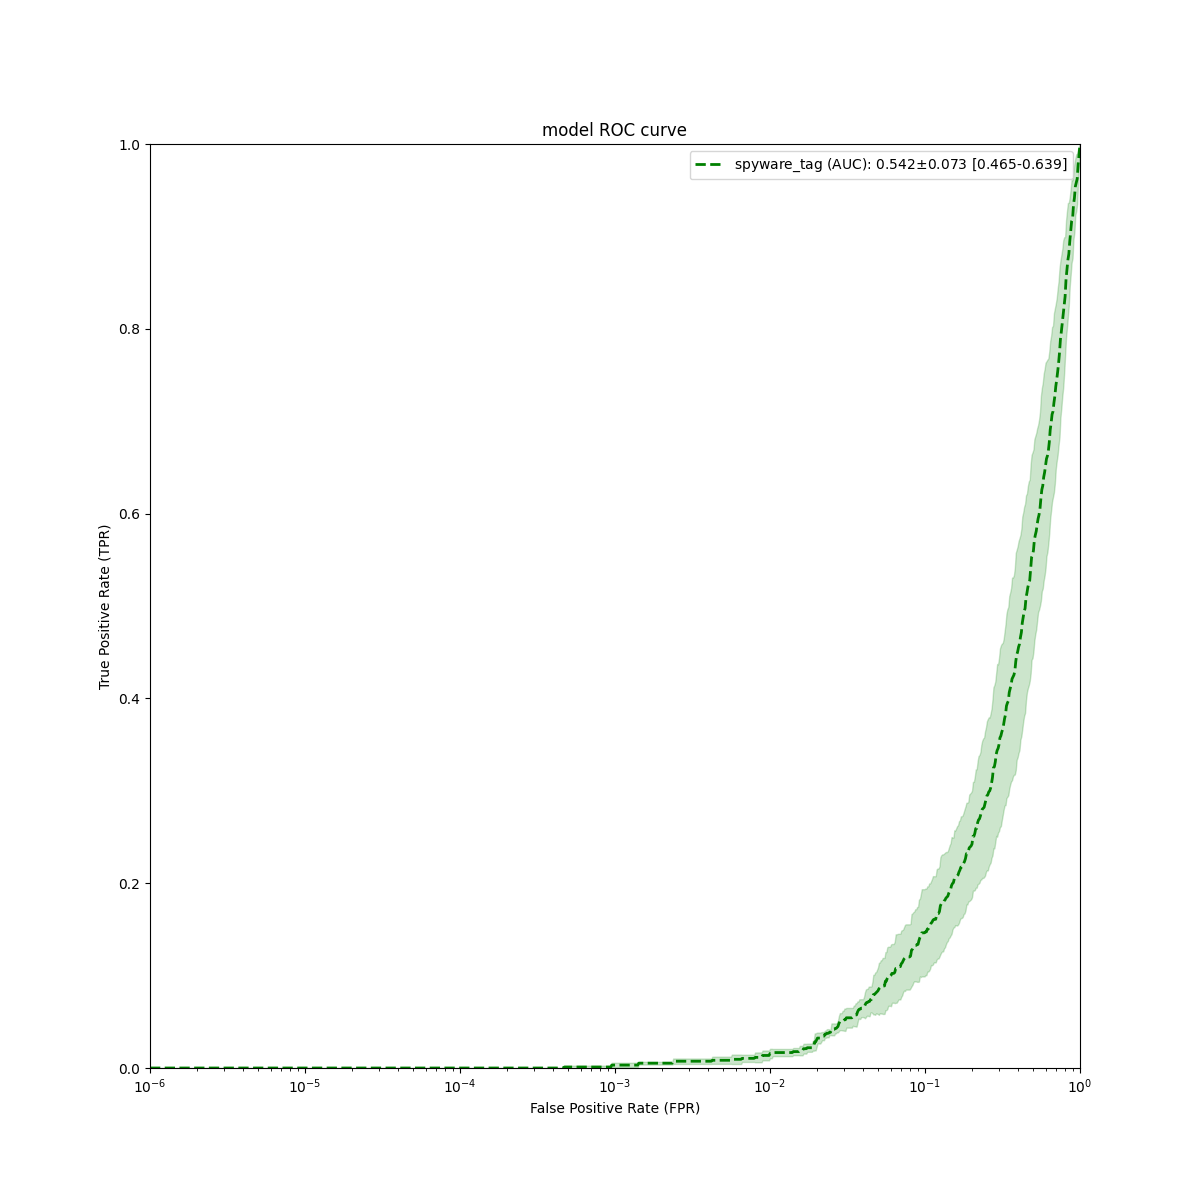
\includegraphics[width=0.6\textwidth]{./results/spyware_tag_roc_aloha.png}
        \vspace*{-0.2cm}
        \caption{ROC curve and AUC statistics of \textBF{ALOHA} model for the \textbf{Spyware Tag}. The line represents the \textit{mean} TPR at a given FPR, while the shaded region represents the \textit{standard deviation}. Statistics were computed over \textBF{3} training runs, each with random parameter initialization.}
        \label{fig:spywareTagRocAloha}
    \end{figure}
}

\newcommand{\spywareTagRocJointEmbedding}{
    \begin{figure}[H]
        \vspace*{-0.5cm}
        \centering
        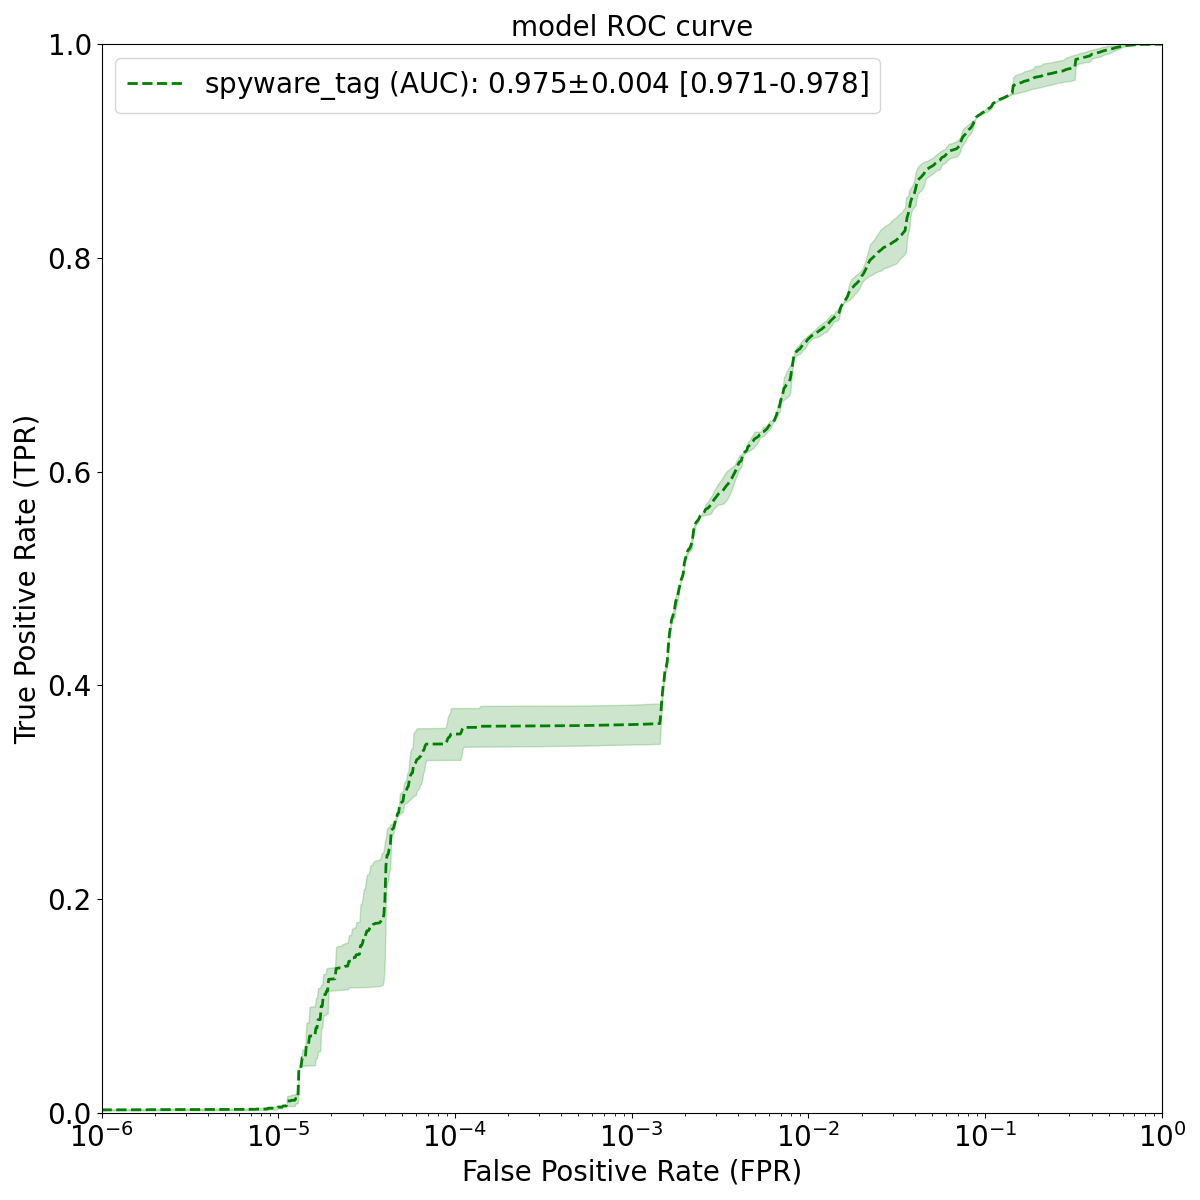
\includegraphics[width=0.6\textwidth]{./results/spyware_tag_roc_jointEmbedding.png}
        \vspace*{-0.2cm}
        \caption{ROC curve and AUC statistics of \textBF{Joint Embedding} model for the \textbf{Spyware Tag}. The line represents the \textit{mean} TPR at a given FPR, while the shaded region represents the \textit{standard deviation}. Statistics were computed over \textBF{3} training runs, each with random parameter initialization.}
        \label{fig:spywareTagRocJointEmbedding}
    \end{figure}
}

\newcommand{\spywareTagRocProposedMethod}{
    \begin{figure}[H]
        \vspace*{-0.5cm}
        \centering
        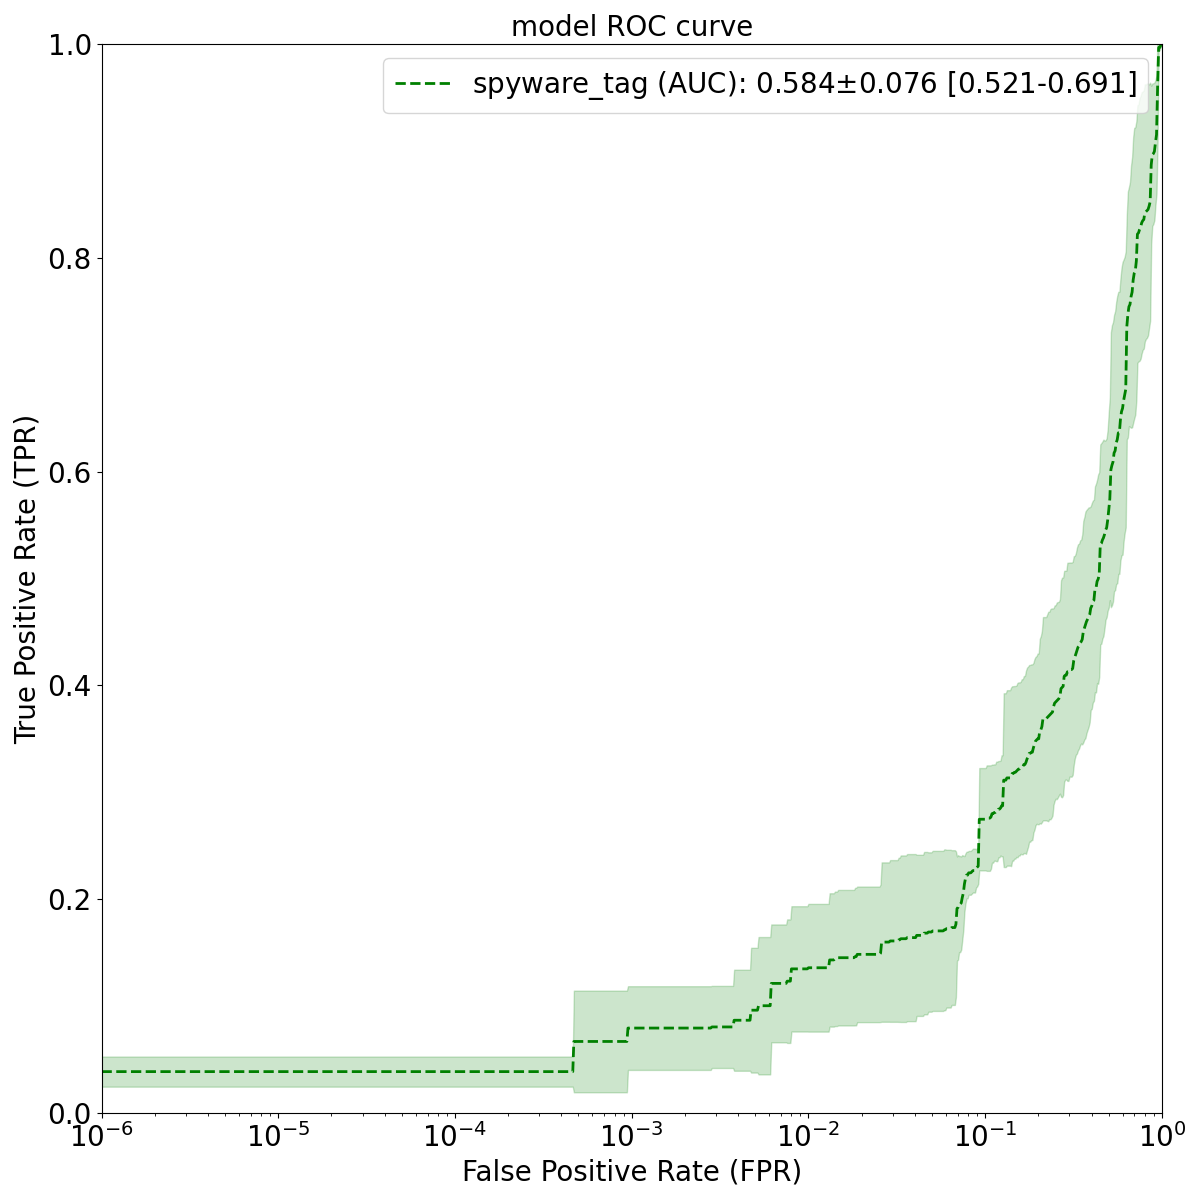
\includegraphics[width=0.6\textwidth]{./results/spyware_tag_roc_proposedModel.png}
        \vspace*{-0.2cm}
        \caption{ROC curve and AUC statistics of \textBF{Proposed Model} for the \textbf{Spyware Tag}. The line represents the \textit{mean} TPR at a given FPR, while the shaded region represents the \textit{standard deviation}. Statistics were computed over \textBF{3} training runs, each with random parameter initialization.}
        \label{fig:spywareTagRocProposedModel}
    \end{figure}
}
